%This work is licensed under the Creative Commons License Attribution 4.0 International (CC-BY 4.0)
%https://creativecommons.org/licenses/by/4.0/legalcode
\documentclass[rgb]{standalone}
\usepackage{tkz-euclide}
\usepackage{amsmath}
\definecolor{myorange}{hsb}{0.0833, 1, 0.8}
\definecolor{mygreen}{hsb}{0.3333, 1, 0.8}
\definecolor{myblue}{hsb}{0.5833, 1, 0.8}
\definecolor{mymagenta}{hsb}{0.8333, 1, 0.8}
\begin{document}
	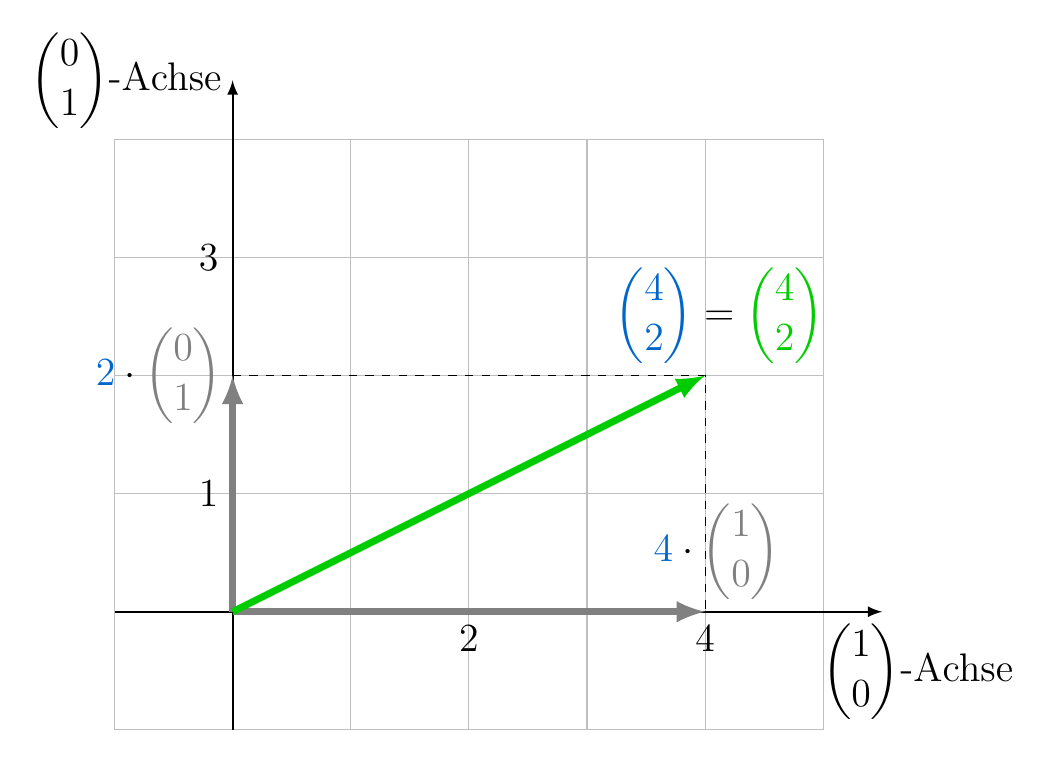
\begin{tikzpicture}[scale=1.5, font=\Large]
		% Coordinate system
		\tkzInit[xmin=-1,xmax=5,ymin=-1,ymax=4]
		\tkzGrid[color=lightgray]
		\tkzDrawX[thick, label=$$]
		\tkzDrawY[thick, label=$\begin{pmatrix} 0 \\ 1 \end{pmatrix}$-Achse]
		\draw[dashed] (0,2) -- (4,2) -- (4,0);
		\draw[line width=2.5pt, gray, -latex] (0,0) -- (4,0);
		\draw[line width=2.5pt, gray, -latex] (0,0) -- (0,2);
		\draw[line width=2.5pt, mygreen, -latex] (0,0) -- (4,2);
		% Labels
		\node[left=0.5mm] at (0,1){$1$};
		\node[left=0.5mm] at (0,3){$3$};
		\node[below=0.5mm] at (2,0){$2$};
		\node[below=0.5mm] at (4,0){$4$};
		\node[above right] at (3.15,2){${\color{myblue}{\begin{pmatrix} 4 \\ 2 \end{pmatrix}}}=\color{mygreen}{\begin{pmatrix} 4 \\ 2 \end{pmatrix}}$};
		\node[above] at (4.1,0){${\color{myblue}{4}}\cdot\color{gray}{\begin{pmatrix} 1 \\ 0 \end{pmatrix}}$};
		\node[left] at (0,2){${\color{myblue}{2}}\cdot\color{gray}{\begin{pmatrix} 0 \\ 1 \end{pmatrix}}$};
		\node[below] at (5.8,0){$\begin{pmatrix} 1 \\ 0 \end{pmatrix}$-Achse};
	\end{tikzpicture}	
\end{document}